\section{Generating meshes}\label{sec:meshGeneration}
A simulation begins with a mesh file describing the specimen geometry, volume elements and region IDs. Simple specimens can be generated with \href{https://gmsh.info/}{Gmsh}; more elaborate polycrystalline specimens can be generated with \href{https://neper.info/}{Neper}. After generation, MoDELib reads the mesh and constructs the connectivity and grain-boundary topology used by the simulation.

\subsection{Simple geometries with Gmsh}
Gmsh provides geometry definition and finite-element mesh generation. For cubes, cylinders and simple partitions, start from the geometry files \code{Library/Meshes/unitCube.geo}, \code{cylinder.geo} or \code{bicrystal.geo}. For example, from the repository root:
\begin{lstlisting}[language=bash,basicstyle=\footnotesize\ttfamily]
gmsh Library/Meshes/unitCube.geo -3 -order 1 -format msh2 -o mesh.msh
\end{lstlisting}
This writes a tetrahedral mesh to \code{mesh.msh}; changing the geometry's size parameters changes the discretization. The current reader uses ASCII Gmsh version 2 records and takes the second element tag as the region ID. Preserve distinct volume entities for different grains. See the \href{https://gmsh.info/doc/texinfo/gmsh.html}{Gmsh reference manual} for geometry and meshing options.

\subsection{Polycrystals and periodicity with Neper}
Neper generates grain tessellations and meshes them, including periodic and partially periodic polycrystals. Its tessellation and meshing stages are separate:
\begin{lstlisting}[language=bash,basicstyle=\footnotesize\ttfamily]
neper -T -n 10 -periodicity all -o poly10
neper -M poly10.tess -order 1 -format msh:ascii
\end{lstlisting}
These commands illustrate a ten-grain periodic tessellation and its mesh; they are not recipes for reproducing a particular stored library file. Neper's meshing stage uses Gmsh for tetrahedral meshing. The \href{https://neper.info/doc/neper_t.html}{tessellation documentation} describes grain morphology and periodicity, and the \href{https://neper.info/doc/neper_m.html}{meshing documentation} describes element size and output formats.

Neper's periodicity selector accepts all directions or a subset of its generation axes, such as \code{x,y}. Periodic directions in the simulation need not align with the global Cartesian axes: rotate a periodic mesh into the desired frame, or apply the nonsingular import transformation $\bm F$ introduced below. A source translation $\bm a_k$ then becomes $\bm F\bm a_k$, allowing oblique directions as well. The same transformation must act on the whole mesh so that paired nodes and triangulations still match. MoDELib activates the desired geometric pairing when the mesh is constructed; generating a periodic file alone does not select a field boundary condition.

\subsection{Examples in the mesh library}
Figure~\ref{fig:meshLibrary} shows four existing files from \code{Library/Meshes}. The cube and cylinder provide single-region examples; the bicrystal introduces a grain boundary. The ten-grain periodic unit has a jagged exterior following whole grains, and translated copies fill space. Its exterior is not a cut through grains at the boundary of a rectangular box.
\begin{figure}[t]
\centering
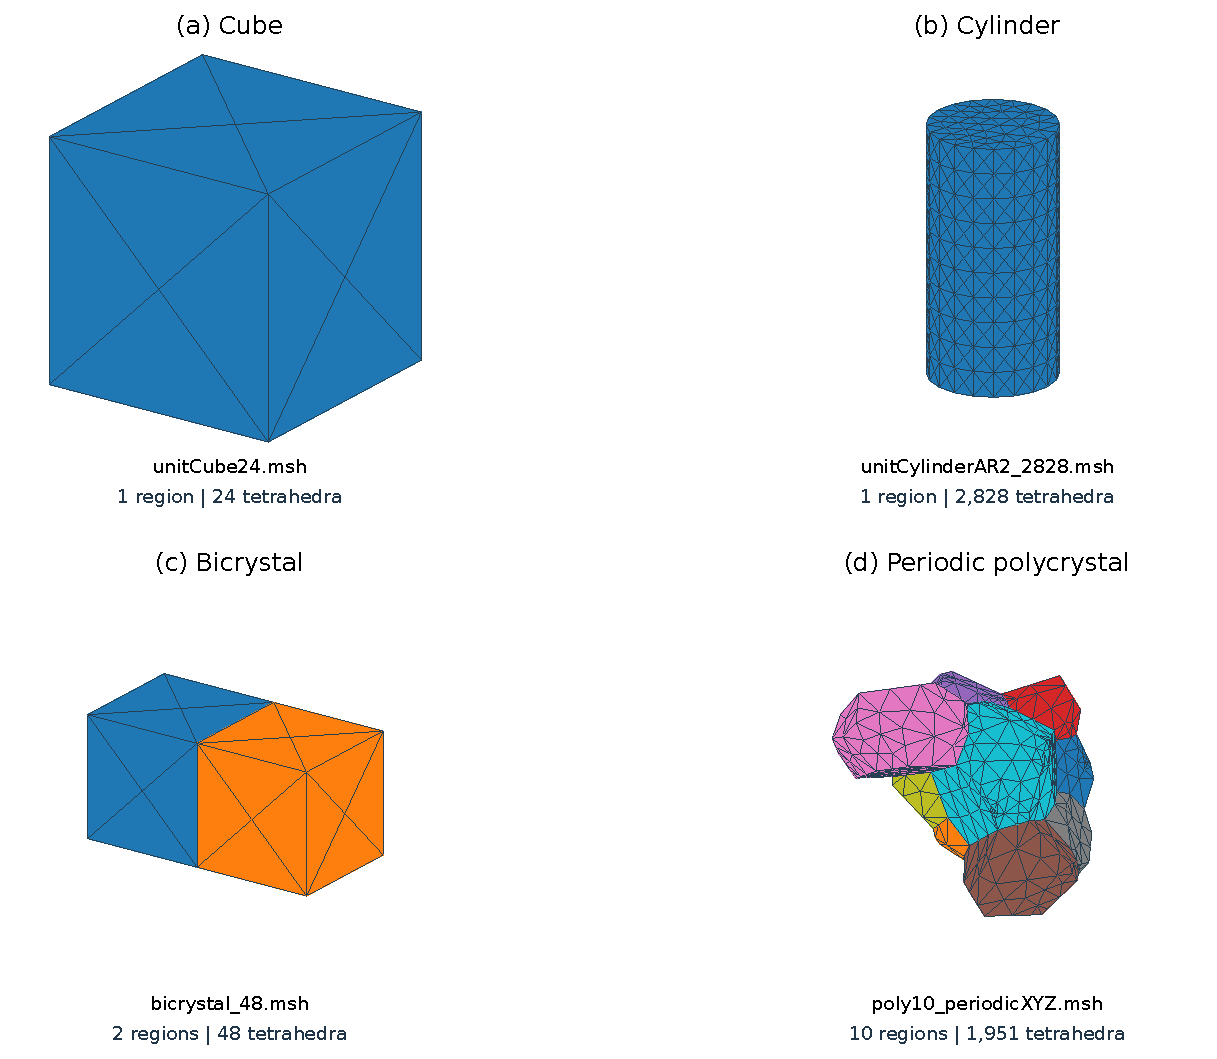
\includegraphics[width=0.98\textwidth]{mesh_library_examples}
\caption{Existing volume meshes in \code{Library/Meshes}, displayed through their exterior triangulations. Colors identify region IDs. Each specimen is scaled independently for display; counts refer to volume tetrahedra. Quadratic edge nodes, when present in the source file, are omitted from the sketches.}\label{fig:meshLibrary}
\end{figure}
Further examples include \code{polycrystalCube_10_periodicX.msh}, \code{polycrystalCube_10_periodicXY.msh}, \code{poly30_periodicXYZ.msh} and \code{polycrystalCyl_50.msh}. Select a file with the geometry, grain structure and matching periodic boundaries required by the problem, then check its region IDs against the material input.
\sourcefile{src/Mesh/SimplexReader.cpp}
